\leadauthor{theRmal-landscape}

\title{Variation in thermal pressures and resource availability drives disease dyanmics}
\shorttitle{theRmal-landscape}

\author[1]{
  
% \orcidlink{0000-0001-0000-0000}
}
% \author[2]{Second Doctor \orcidlink {000-0002-0000-0000}}
% \author[1,\Letter]{Third Professor \orcidlink {000-0003-0000-0000}}
% \affil[1]{A University, Academic Street, Learningtown, UK}
% \affil[2]{B Institute, Chalk Road, Blackboardville, USA}
\date{}

\maketitle

\begin{abstract}
Abstract of the paper goes here.
\lipsum[1]
\end{abstract}

\begin{keywords}
keyword1 | keyword2 | keyword3
\end{keywords}

\begin{corrauthor}
% third.professor\at awesome.ac.uk
\end{corrauthor}

\section*{Introduction}\label{s:introduction}

\begin{itemize}
    \item Direct transmission of infectious disease is driven largely by physical proximity between infected hosts and susceptible hosts. 
    \item Physical proximity can be driven by complex social dynamics, but in a simplified framework is most easily described by the probability that organisms making foraging choices on a landscape chose the same patch and then subsequently a transmission event occurs
    \item Foraging choices on a landscape is driven largely by resource availability
    \item In an environment where organisms are sensitive to the thermal landscape as well, choices will be made not just based on resource availability but on the thermal suitability of various patches
    \item A simplified landscape can therefore be thought of as jointly described by the thermal and resource properties of a given patch 
    \item Transmission dynamics on a landscape will therefore be characterized by these factors as well
    \item In this simplified framework then, the probability of a single infected individual transmitting a generalized pathogen to another individual is modulated by the thermal and resource landscapes
    \item A biological motivation of this is to consider some burrowing organisms which directly transmit a pathogen of interest between them, dependent on physical proximity
\end{itemize}

\section*{Methods \& Results}\label{s:methods-results}

To abstract the transmission dynamics sufficiently, we imagine a landscape where a series of individuals make daily landscape-level selections on where they will forage, with no memory and perfect knowledge of the landscape. Therefore, they chose from the available cells, $w_i$ based on each cell's value as a probability. Since these are probabilities it must be true that 
\begin{equation}
\sum_i w_{i}=1.
\end{equation}

If there are $S$ susceptible individuals in the population that assort randomly across space according to the probabilities $w_{i}$ and $I=1$ infected individual, we want to know the probability that the disease will spread. From a purely contact perspective, this is given by the probability that the infected individual occupies a location that also has at least one susceptible individual.

\subsection{Co-location and transmission}

Assuming a population consisting of $S>0, I>0$, transmission requires at least the co-location of one of each group. We can consider both co-location and transmission.

\subsubsection{Determining the probability that at least one $S$ is located in a cell $i$}

The probability that patch $i$ has zero susceptible individuals is $P(S_{i}=0)=(1-w_{i})^S$, where $S$ is the number of susceptible individuals on the landscape. Thus, the probability that at least one patch at location $i$ has at least one susceptible individual is given by:  
\begin{align}
P(s_{i} \geq 1) &=1-P(s_{i}=0) \\
&=P(s_{i}=1)+P(s_{i}=2)+P(s_{i}=3)+ ... +P(s_{i}=S)
\end{align}
Each of the terms above can be expanded as follows: 
\begin{align}
P(s_{i}=k)=\binom{S}{k}w_{i}^k(1-w_{i})^{S-k}
\end{align}
and therefore
\begin{align}
P(s_{i} \geq 1)&=\sum_{k=1}^{S}\binom{S}{k}w_{i}^k(1-w_{i})^{S-k}\\
&=\left((1-w_{i})^{-S}-1\right)(1-w_{i})^S\\
&=1-(1-w_{i})^S
\end{align}

\subsubsection{Joint Probability for Co-location of $S$ and $I$}
For disease spread to occur, both a susceptible individual and an infected individual must be in the same cell. The probability of this is the product of the independent events:
\begin{equation}
P(\text{collocation in cell } i) = P(S_{i} \geq 1) \cdot P(I_{i} \geq 1).
\end{equation}

Expanding this:
\begin{equation}
P(\text{collocation in cell } i) = \left[ 1 - (1 - w_{i})^S \right] \cdot \left[ 1 - (1 - w_{i})^I \right].
\end{equation}

\subsection{Landscape with a known distribution}

In above formulations, the landscape values $w$ are a function of both $T$ and $R$, however, we can make a further simplifying assumption in some cases that the values, while implicitly still based on $T$ and $R$ are instead given by some known distribution. The landscape on which individuals are making occupancy decisions can be thought of as consisting of normalized values, where the number of patches $n$ is sufficiently large. We also focus on the case where there is only one $I$ individual and transmission is assured by co-occurring on the landscape.

We begin considering that $w$ takes a uniform random distribution. We assume that the quality $q_i$ of each patch is drawn at random from a uniform distribution $(0,1)$, and then transform these qualities to get patch weights $w_i$ by dividing each patch by the total of the quality values where $i = 1,...,n$. 

\begin{equation}
    w_i = \frac{q_i}{\sum_i{q_i}}
\end{equation}

Here, $w_i$ are therefore nearly uniformly distributed 
\begin{equation}
    (0, \frac{2}{n})
\end{equation} 
for large enough $n$. Here we are considering the case where co-location by two $S$ individuals is given by 
\begin{equation}
    n*w(1-(1-w)^S).
\end{equation} 

If we assume that $n>2$ and also that $S \geq 1$, then the expectation of our co-location is: 

\begin{equation}
    E[n*w(1-(1-w)^S)] = \frac{n^{-S} \left(\left(2 (S+1) (S+2)-n^2\right) n^S+(n-2)^{S+1} (n+2
   S+2)\right)}{2 (S+1) (S+2)}. 
\end{equation}

If we compare this set of expected values, varying the ratio of $S/n$, then we can see our expected values match the draws from a simulated distribution 

\begin{figure}
    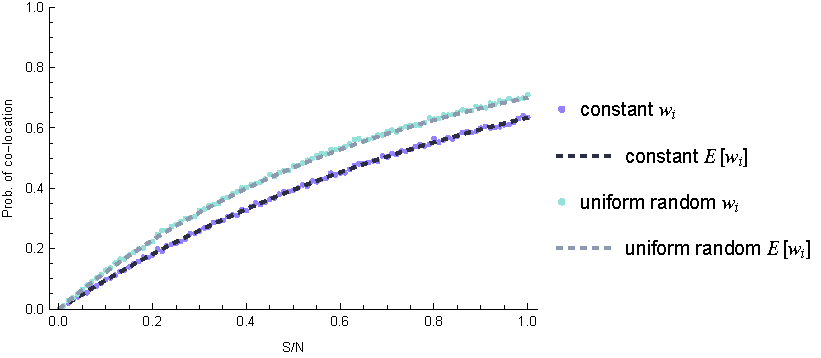
\includegraphics[width=0.75\linewidth]{figs/si/constant-uniform.pdf}
\end{figure}

We could also assume that the weights are exponentially distributed, since $n$ random draws from an exponential with a mean $\frac{1}{\lambda} = 1$ would sum to a mean of 1, given large enough $n$. That would take the form 

\begin{equation}
    E[n*w(1-(1-w)^S)] = \frac{1-n^2+S-\mathcal{e}^{-n}(-n)^{-S}(1+n+S)((-1+(-1)^{2S}) \Gamma(2+S)+\Gamma(2+S, -n))}{1+S}
\end{equation}


\subsubsection{Probability of Successful Transmission}

To determine whether or not transmission can occur, we consider the case where infected and susceptible individuals are present on the same landscape patch, and also the likelihood of a transmission event occurring successfully. We denote this as $\epsilon(T)$ which is the temperature dependent probability of transmission.  Given some collocation, if there is some patch with $S = 1, I = 1$, the likelihood of transmission is just $\varepsilon_{i}(T)$. In the case of $S = 2$, we have the probability of 
\begin{align}
    \text{At least one S getting infected} &\rightarrow 1 - (1- \varepsilon(T))^2, \\
    \text{Both } S \text{ getting infected} &\rightarrow \varepsilon(T)^2, \text{and} \\
    \text{Neither } S \text{ getting infected} &\rightarrow (1 - \varepsilon(T))^2
\end{align}

\subsubsection{Some $k$ number of susceptible individual and one infected}

If there is only $I = 1$ then the probability of at least one of the susceptible $k$ undergoing infection, $P^*(S, I)$ is

\begin{equation}
    P^*(k, I=1) = \sum^{k=S}_{k = 1}\begin{pmatrix} S\\ k \end{pmatrix} w(T)^{k-1}(1-w(T))^{S-k}(1 - (1-\varepsilon(T))^k)
\end{equation}

From there, we can understand that the probability of a disease spreading on the landscape from cell $i$, $\phi_{i}(k, I = 1)$ is 

\begin{equation}
    \phi_{i}(k, I = 1) = 1 - (1 - w(T) \varepsilon(T))^S
\end{equation}

And therefore the probability of it spreading on the landscape at all is:

\begin{equation}
    \boldsymbol{\phi}(k, I = 1) = \sum_i 1 - (1 - w(T) \varepsilon(T))^S
\end{equation}





\begin{equation}
    w_{i} = \text{Max}(0, f(T_{i}, R_{i}))
\end{equation}

where $f(T_{i}, R_{i})$ is the function defining the suitability of patch $i$ based on the resource availability and temperature suitability of patch $i$:

\begin{equation}
    f(T_{i}, R_{i}) = \frac{I_{\text{max}}(T_{i} R_{i})}{R_{i} + R_{\text{half}}} - m(T_{i}),
\end{equation}

with $m(T)$ being a respiration term of the organism, and $I_{\text{max}(T)}$ is the maximum uptake rate, where $m(T) = m_a e^{m_b \times T} + m_c$ and $I_{\text{max}}(T) = e^{-(T - T_I)^2 / \gamma}$ with $m$ being an approximated exponential version of the Boltzmann-Arrhenius relationship. Here $T_I$ is the optimal temperature value and $\gamma$ determines the breadth of the response. This value is dependent on each cell, where $T_{i}$ is the temperature value at $i$ and $R_{i}$ is the inflow supply of some resource for the organism choosing it's location \Cref{fig:t-s-wij-grid}. The values for a given cell of $T$ and $S$ are drawn from:

%\section*{Results}\label{s:results}


%\section*{Discussion}\label{s:discussion}


\section*{Bibliography}
\bibliographystyle{bxv_abbrvnat}
\bibliography{theRmal-landscape.bib}